
\section{Introduction to Excel}

Microsoft Excel is the spreadsheet program we will use for much of our
data analysis and graphing.  It is a powerful and easy-to-use
application for graphing, fitting, and manipulating data. In this
appendix, we will briefly describe how to use Excel to do some useful
tasks.  

\subsection{Data and formulae}

The figure below shows a sample Excel spreadsheet containing data
from a made-up experiment.  The experimenter was trying to measure
the density of a certain material by taking a set of cubes
made of the material and measuring their masses and the lengths of
the sides of the cubes.  The first two columns contain her measured
results.  \textbf{Note that the top of each column contains both
a description of the quantity contained in that column and its units.}
You should make sure that all of the columns of your data tables do as well.
You should also make sure that the whole spreadsheet has a descriptive
title and your names at the top.

In the third column, the experimenter has figured out the volume
of each of the cubes, by taking the cube of the length of a side.
To avoid repetitious calculations, she had Excel do this automatically.
She entered the formula ``=B3$\wedge$3'' (without the quotes) into cell C3.
Note the equals sign, which indicates to Excel that a formula is coming.
The $\wedge$ sign stands for raising to a power.  After entering a formula
into a cell, you can grab the square in the lower right corner of the
cell with the mouse and drag it down the column.  This will copy
the cell, making the appropriate changes, into the rest of the column.
For instance, in this case, cell C4 contains the formula ``=B4$\wedge$3,''
and so forth.

Column D was similarly produced with a formula that divides the
mass in column A by the volume in column C.

At the bottom of the spreadsheet we find the mean and standard
deviation of the calculated densities (that is, of the numbers
in cells D3 through D6).  Those are computed
using the formulae ``=average(D3:D6)'' and ``=stdev(D3:D6)''.

{\par\centering \resizebox{5in}{!}{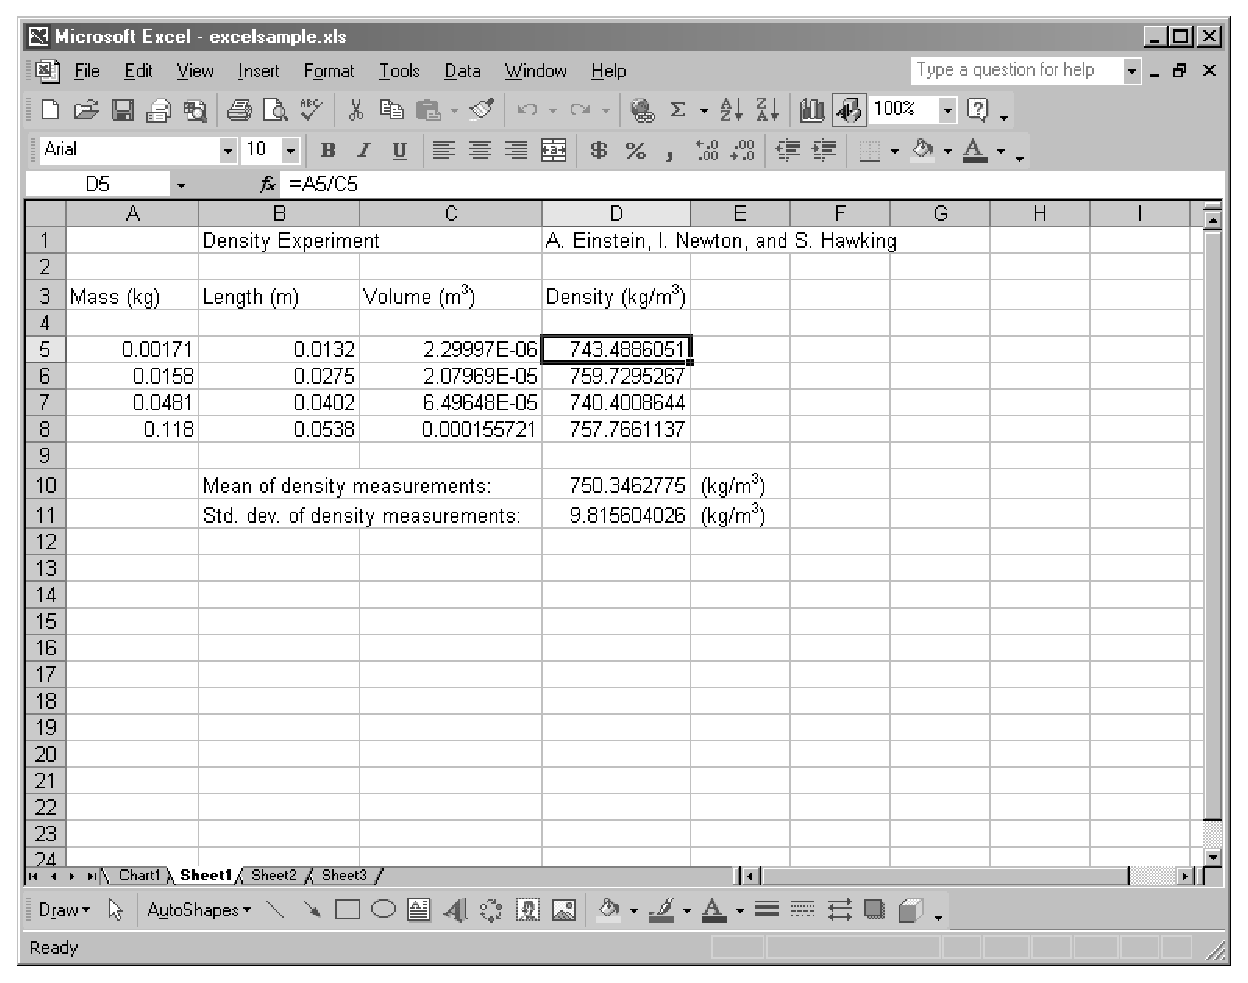
\includegraphics{excelwindow.eps}} \par}


\subsection{Graphs}

Making graphs in Excel is relatively easy.  First, use the mouse
to select the columns of numbers you want to graph.  (If the two
columns aren't next to each other, select the first one, then hold
down the control key while selecting the second one.)
Then click on the ``chart wizard'' button (which looks like this

\includegraphics{bargraph.eps}).  

There are a number of different styles of graphs that the chart wizard
can generate.  In nearly every case, you will want to select an
``XY (scatter)'' graph.  Click ``Next'' to proceed to customize
your graph.  The most useful customization options come in step 3
of the process.  Under ``Title,'' you can put appropriate labels
on the $x$ and $y$ axes of your graphs and give the overall graph
a descriptive title.  \textbf{All graphs must have correctly labeled
axes (including units).}  If the graph contains only one set of data
points, you may wish to uncheck the box that says ``Show legend'':
the information in the legend is probably already contained in the
title and axis labels, so the legend just takes up space.

Sometimes, you may want to make a graph in Excel where the $x$ column
is to the right of the $y$ column in your worksheet.  In these cases,
Excel will make the graph with the $x$ and $y$ axes reversed.  There
are at least two ways to fix this problem.  The simplest way is to make
a copy of the $y$ column in the worksheet and paste it so that it's
to the right of the $x$ column.  If you don't want to do that, here's
another way.  In step 2 of the chart wizard, look under the ``Series''
tab.  Click on this icon 
\includegraphics{excelicon.eps} next to the
place where it says ``X values.''  You can now select which column of data you
want to go on the $x$ axis. Do the same thing to select the correct
$y$ column.

\subsection{Fitting lines and curves}

After you've made a graph, you can have Excel draw a straight line or
curve that is a best fit to the data.  Under the ``chart'' menu,
select ``Add trendline.''  The most common sort of trendline you
will add is a linear fit, but you can also have Excel draw other
sorts of best-fit
curves.  Under the ``options'' tab, you can check a box that causes
Excel to display the equation for the line or curve it has drawn.
{\bf Excel will not put the correct units on the numbers in this equation,
but you should.}
